\chapter{Uvod u osnove teorije algoritama}

U ovom poglavlju uvode se osnovni pojmovi teorije algoritama i računanja. Najprije se definiše pojam računarskog problema, zatim pojam algoritma kroz apstraktni model računanja, a potom osnovni koncepti vremenske i prostorne složenosti algoritama. Na kraju se razmatra pitanje ispravnosti algoritama, sa posebnim osvrtom na metodu invarijantne petlje.\\


Nakon uspješnog savladavanja sadržaja ove glave student će biti u stanju da:

\begin{itemize}
	\item definiše računarski problem, instancu problema, rješenje, računarski program i algoritam;
	
	\item razlikuje osnovne vrste računarskih problema i algoritamskih pristupa;
	
	\item objasni osnovne pretpostavke teorijskog RAM modela;
	
	\item odredi veličinu ulaza za jednostavne računarske probleme;
	
	\item analizira broj elementarnih operacija koje algoritam izvršava te odredi vremensku i prostornu složenost jednostavnih algoritama;
	
	\item razumije asimptotske notacije $O$, $\Theta$, $\Omega$ i $o$	pri analizi složenosti;
	
	\item predstavi algoritam korištenjem pseudokoda;
	
	\item objasni pojam ispravnosti algoritma i primijeni metod	invarijante petlje na jednostavne algoritme;
	
 
\end{itemize}

\section{Računarski problem}

\textit{Računarski problem} (eng. \textit{computational problem}) predstavlja zadatak koji je potrebno riješiti uz pomoć računara.

Formalna definicija ovog pojma zahtijeva uvođenje više netrivijalnih teorijskih koncepata, među kojima je i pojam jezika. U opštem slučaju, ulaz računarskog problema može se predstaviti kao binarno kodiran niz, odnosno element skupa $L=\{0,1\}^*$. Izlaz predstavlja rješenje (opet element skupa $L$) koje mora zadovoljiti određena svojstva definisana samim problemom. Drugim riječima, računarski problem određuje skup uslova koje izlaz mora zadovoljiti za svaki dopustiv ulaz.

Ulaz problema često se naziva \textit{instancom problema}, dok se odgovarajući izlaz naziva \textit{rješenjem instance}. Jedan od najpoznatijih primjera računarskog problema jeste problem sortiranja. U ulazu je dat niz objekata dužine $n$, dok je cilj proizvesti uređenu verziju tog niza prema unaprijed definisanom kriterijumu uređenja. Pri tome objekti ne moraju biti brojevi; dovoljno je da je nad njima definisana relacija totalnog uređenja.

Na računarski problem možemo gledati kao na preslikavanje između ulaznih i izlaznih objekata. Ulazi i izlazi mogu biti predstavljeni različitim matematičkim strukturama, kao što su brojevi, skupovi, nizovi ili grafovi. U tom kontekstu govori se o generičkoj instanci problema i odgovarajućem generičkom rješenju.

Prije razmatranja različitih tipova računarskih problema uvedimo pojam grafa, jednog od najvažnijih matematičkih objekata u računarstvu. Graf se može posmatrati kao skup čvorova povezanih granama (linijama). U ovoj knjizi podrazumijevamo proste grafove, odnosno grafove koji ne sadrže petlje niti višestruke grane između istog para čvorova. Graf je \textit{usmjeren} ukoliko svaka grana ima pridružen smjer, odnosno uređeni par krajnjih čvorova. U suprotnom, graf se naziva \textit{neusmjerenim}. Primjeri usmjerenog i neusmjerenog grafa prikazani su na Slici~\ref{fig:graphs}.

%graphs

\begin{figure}[ht]
	\centering
	
	\begin{tikzpicture}[
		vertex/.style={
			circle,
			draw,
			minimum size=7mm,
			inner sep=0pt
		},
		edge/.style={
			thick
		},
		directed/.style={
			thick,
			->,
			>=Stealth
		}
		]
		
		% =====================================================
		% Neusmjereni graf
		% =====================================================
		
		\node[vertex] (u1) at (0,2) {$1$};
		\node[vertex] (u2) at (2,2) {$2$};
		\node[vertex] (u3) at (0,0) {$3$};
		\node[vertex] (u4) at (2,0) {$4$};
		
		\draw[edge] (u1) -- (u2);
		\draw[edge] (u1) -- (u3);
		\draw[edge] (u2) -- (u3);
		\draw[edge] (u2) -- (u4);
		\draw[edge] (u3) -- (u4);
		
		\node at (1,-0.8) {\textbf{(a) Neusmjereni graf}};
		
		
		% =====================================================
		% Usmjereni graf
		% =====================================================
		
		\node[vertex] (d1) at (5,2) {$1$};
		\node[vertex] (d2) at (7,2) {$2$};
		\node[vertex] (d3) at (5,0) {$3$};
		\node[vertex] (d4) at (7,0) {$4$};
		
		\draw[directed] (d1) -- (d2);
		\draw[directed] (d1) -- (d3);
		\draw[directed] (d3) -- (d2);
		\draw[directed] (d2) -- (d4);
		\draw[directed] (d4) -- (d3);
		
		\node at (6,-0.8) {\textbf{(b) Usmjereni graf}};
		
	\end{tikzpicture}
	
	\caption{Primjeri neusmjerenog i usmjerenog grafa.}
	\label{fig:graphs}
\end{figure}

Postoji više vrsta računarskih problema. U nastavku izdvajamo četiri najčešće klase koje se pojavljuju u literaturi: probleme odlučivanja, probleme pretraživanja, probleme optimizacije i probleme prebrojavanja.

Problem \textit{odlučivanja} zahtijeva odgovor tipa DA/NE (\emph{True}/\emph{False}) za dati ulaz $x \in \{0,1\}^*$. Drugim riječima, potrebno je utvrditi da li ulazna instanca posjeduje određeno svojstvo. Kao primjer može poslužiti problem \textit{3-bojenja} grafa (3--COL). U ulazu je dat neusmjereni graf, a potrebno je odrediti da li postoji dodjela boja iz skupa ${1,2,3}$ svim čvorovima tako da nijedna dva susjedna čvora nemaju istu boju.

Prikladan način formalizacije problema odlučivanja jeste određivanje skupa svih ulaza za koje je odgovor potvrdan. Takav skup označavamo sa $L \subseteq \{0,1\}^*$ i nazivamo ga jezikom. Na taj način svaki problem odlučivanja može biti predstavljen odgovarajućim jezikom, a svaki jezik određuje jedan problem odlučivanja. Na primjer, skup svih 3-obojivih grafova predstavlja jezik koji opisuje problem 3-bojenja.

Kod problema \textit{pretraživanja}, za dati ulaz $x \in \{0,1\}^*$ potrebno je pronaći objekat $y \in \{0,1\}^*$ koji zadovoljava određeni odnos sa ulazom. Takvi problemi formalizuju se relacijom $R \subseteq \{0,1\}^* \times \{0,1\}^*$, pri čemu $(x,y)\in R$ označava da je $y$ dopustivo rješenje za instancu $x$.

Posmatrajmo ponovo problem 3-bojenja. Neka je dat neusmjereni graf $G=(V,E)$. Potrebno je pronaći, ukoliko postoji, funkciju bojenja $c \colon V \rightarrow \{1,2,3\}, 
$ takvu da za svaku granu $(u,v)\in E$ važi $c(u)\neq c(v)$. Za razliku od verzije odlučivanja, ovdje nije dovoljno utvrditi postojanje rješenja; potrebno je i eksplicitno konstruisati jedno takvo rješenje.

Problemi \textit{optimizacije} predstavljaju jednu od najvažnijih klasa računa\-rskih problema. Glavni cilj je pronalaženje najboljeg rješenja iz skupa svih dopustivih rješenja prema unaprijed definisanoj funkciji cilja koja daje apsolutnu mjeru ``kvaliteta'' svakog rješenja. U zavisnosti od problema, ciljna funkcija se maksimizuje ili minimizuje uz poštovanje zadanih ograničenja.

Klasičan primjer predstavlja problem trgovačkog putnika. Potrebno je pronaći najkraću kružnu rutu (konturu) koja prolazi kroz sve zadate gradove (čvorovi grafa) tačno jednom i vraća se u početni grad. Cilj je minimizovati ukupnu pređenu udaljenost.

Problemi \textit{prebrojavanja} bave se određivanjem broja mogućih rješenja određenog problema. Njihova složenost može varirati od veoma jednostavnih primjera do izuzetno zahtjevnih kombinatornih zadataka.  Pretpostavimo da raspolažemo sa četiri košulje i tri para pantalona različitih boja. Na koliko različitih načina se osoba može obući ukoliko bira jednu košulju i jedne pantalone? Primjenom principa množenja dobijamo da je ukupan broj mogućih kombinacija jednak  $
4 \cdot 3 = 12.
$ Za kraj ovog poglavlja dajemo formalnu definiciju računarskog problema.

\begin{definition}
	Računarski problem je funkcija 	$
	f \colon \Sigma^* \rightarrow 2^{\Sigma^*}.
	$ Za dati ulaz $x$, skup $f(x)$ predstavlja skup svih ispravnih odgovora za instancu $x$.
\end{definition}

\section{Računarski program i pojam algoritma}

Računarski program predstavlja konačan niz instrukcija koje računar može izvršavati. Instrukcije određuju redoslijed operacija potrebnih za rješa\-vanje određenog problema ili izvršavanje konkretnog zadatka. Programi mogu biti namijenjeni obradi teksta, analizi podataka, pretraživanju informacija na internetu, komunikaciji sa korisnikom, upravljanju uređajima ili brojnim drugim primjenama.

Programi se izvršavaju na različitim platformama, uključujući personalne računare, mobilne uređaje, serverske sisteme i ugrađene računarske uređaje. Za njihovu implementaciju koriste se različiti programski jezici, među kojima su Pajton, Java, $ C$, $ C$++ itd. Nakon što je program napisan, potrebno ga je prevesti u mašinski k\^od razumljiv procesoru. U zavisnosti od programskog jezika i načina izvršavanja, taj proces može uključivati kompajliranje, interpretaciju ili kombinaciju oba pristupa.

Algoritam predstavlja precizno definisan konačan niz koraka kojim za dati ulaz proizvodi odgovarajući izlaz, odnosno rješava određeni problem. U informatici se algoritmi koriste kao formalni opisi postupaka koje računarski program izvršava kako bi ostvario željenu funkcionalnost.

Može se posmatrati kao recept za rješavanje problema: algoritam definiše koje operacije treba izvršiti, kojim redoslijedom i pod kojim uslovima. Jednostavna analogija iz svakodnevnog života jeste priprema jela prema receptu. Recept opisuje niz koraka koje je potrebno izvršiti kako bi se od početnih sastojaka dobio željeni rezultat. Na sličan način algoritam transformiše ulazne podatke u odgovarajući izlaz.

Primjeri dobro poznatih algoritama uključuju algoritme sortiranja, koji uređuju podatke prema zadatom kriterijumu, algoritme pretraživanja za pronalaženje informacija u velikim skupovima podataka, algoritme kompresije i dekompresije podataka, kao i algoritme koji se koriste u kriptografiji i zaštiti informacija.

Uloga algoritama u računarstvu je višestruka:

\begin{itemize}
	\item Omogućavaju efikasno rješavanje složenih problema.
	\item Predstavljaju osnovu automatizacije procesa, čineći ih bržim, pouzdanijim i jednostavnijim za izvršavanje.
	\item Omogućavaju računarima izvršavanje zadataka koje bi čovjek teško ili praktično nemoguće mogao obaviti ručno u realnom vremenu.
\end{itemize}

Međutim, svaki niz instrukcija ne predstavlja nužno algoritam. Da bi određeni postupak bio algoritam, potrebno je da zadovoljava nekoliko osnovnih osobina:

\begin{itemize}
	\item \textit{Dobro definisani ulazi}. Ukoliko algoritam koristi ulazne podatke, oni moraju biti jasno definisani i unaprijed određeni.
	\item \textit{Dobro definisani izlazi}. Za svaki dopustiv ulaz algoritam mora proizvesti jasno određen rezultat.
	\item \textit{Konačnost}. Algoritam mora završiti nakon konačnog broja koraka za svaki dopustiv ulaz.
	\item \textit{Izvodljivost}. Svaka operacija algoritma mora biti izvršiva unutar raspoloživih računarskih resursa.
	\item \textit{Nezavisnost od programskog jezika}. Algoritam predstavlja apstraktan postupak koji se može implementirati u različitim programskim jezicima.
	\item \textit{Nedvosmislenost}. Svaka instrukcija mora biti precizno definisana i jednoznačno interpretirana.
\end{itemize}

Navedene osobine mogu se sažeti kroz nekoliko ključnih karakteristika algoritama:

\begin{itemize}
	\item Algoritam se završava u konačnom vremenu.
	%\item Za dati ulaz proizvodi odgovarajući deterministički izlaz.
	\item Za isti ulaz daje isti izlaz/rezultat, pod pretpostavkom determinističkog izvršavanja.
	\item Svaki njegov korak predstavlja efektivnu i izvršivu operaciju.
\end{itemize}

\textit{Veličina ulaza} predstavlja mjeru količine podataka koje algoritam obra\-đuje. Način određivanja dimenzije ulaza zavisi od prirode problema. Kod problema sortiranja veličina ulaza odgovara broju elemenata koji se sortiraju. Kod problema nad grafovima može se definisati brojem čvorova i grana, dok se kod numeričkih problema često izražava brojem bitova potrebnih za predstavljanje ulaznih vrijednosti.

\subsection{Vrste algoritama}

Tokom razvoja računarstva razvijen je veliki broj algoritamskih paradigmi za rješavanje različitih klasa problema. U nastavku navodimo neke od najvažnijih pristupa koji će biti detaljnije obrađeni u kasnijim poglavljima.

\begin{enumerate}
	\item \textit{Iscrpna pretraga} (eng. \emph{brute force}) predstavlja jedan od najjednostavnijih pristupa rješavanju problema. Osnovna ideja sastoji se u razmatranju svih mogućih kandidata za rješenje i provjeri koji od njih zadovoljavaju uslove problema.
	
	\item \textit{Rekurzivni algoritmi} (eng. \textit{recursive algorithms}) zasnivaju se na razlaganju problema na manje podprobleme istog tipa. Rješenje se dobija ponovnim pozivanjem iste procedure sve dok se ne dostigne trivijalan slučaj koji se može direktno riješiti.
	
	\item \textit{Vraćanje unazad} (eng. \emph{backtracking}) predstavlja tehniku sistematskog pretraživanja prostora rješenja. Kandidati za rješenje grade se postepeno, pri čemu se djelimična rješenja koja ne mogu dovesti do validnog konačnog rješenja odbacuju čim se to utvrdi.
	
	\item \textit{Algoritmi pretraživanja} (eng. \textit{search algorithms}) koriste se za pronalaženje elemenata ili informacija unutar određene strukture podataka.
	
	\item \textit{Algoritmi sortiranja} (eng. \textit{sorting algorithms}) uređuju podatke prema unaprijed definisanom kriterijumu uređenja.
	
	\item \textit{Podijeli pa vladaj} (eng. \emph{divide-and-conquer}) razlaže problem na manje podprobleme, nezavisno ih rješava i zatim kombinuje njihova rješenja u konačan rezultat.
	
	\item \textit{Pohlepni algoritmi} (eng. \textit{greedy algorithms}) grade rješenje korak po korak birajući u svakom trenutku lokalno najpovoljniju odluku prema unaprijed definisanom kriterijumu.
	
	\item \textit{Dinamičko programiranje} (eng. \textit{dynamic programming}) koristi već izračunata rješenja podproblema kako bi se izbjegla višestruka izračunavanja istih vrijednosti. Posebno je efikasno kod problema sa preklapajućim podproblemima i optimalnom podstrukturom.
\end{enumerate}

Većina navedenih pristupa predstavlja opšte algoritamske paradigme koje se mogu primijeniti na širok spektar problema. U trećoj glavi knjige detaljno će biti obrađene najvažnije paradigme, zajedno sa njihovim teorijskim osnovama i praktičnim primjenama.

Projektovanje efikasnih algoritama često predstavlja složen i kreativan proces koji zahtijeva dobro razumijevanje problema, poznavanje postojećih tehnika i sposobnost prepoznavanja odgovarajućih obrazaca rješavanja. Upravo zbog toga algoritamske paradigme imaju značajnu ulogu, jer pružaju opšte strategije koje se mogu prilagoditi velikom broju različitih problema.


\section{Teorijski RAM model}

Prilikom projektovanja i analize algoritama prirodno se nameće nekoliko važnih pitanja:

\begin{enumerate}
	\item Da li je algoritam dovoljno efikasan?
	\item Kako uporediti efikasnost dva različita algoritma za isti problem?
	\item Kako se vrijeme izvršavanja algoritma ponaša kada veličina ulaza postane veoma velika?
\end{enumerate}

Odgovor na ova pitanja zahtijeva precizan i nepristrasan  matematički okvir za opisivanje procesa računanja. Zbog toga se u teorijskoj analizi algoritama uvode apstraktni modeli računara koji omogućavaju formalno mjerenje vremena i prostora potrebnih za izvršavanje algoritama.

Jedan od najčešće korištenih modela jeste \textit{mašina sa slučajnim pristupom} (eng. \textit{Random Access Machine} -- RAM). Ovaj model predstavlja idealizovanu apstrakciju računara koja omogućava formalnu analizu algoritama nezavisno od konkretne hardverske arhitekture.

RAM model pretpostavlja postojanje glavne memorije organizovane kao niz adresabilnih memorijskih ćelija. Svakoj ćeliji može se pristupiti direktno, pri čemu se njen sadržaj može čitati ili mijenjati u konstantnom vremenu. Takođe se pretpostavlja da se instrukcije izvršavaju sekvencijalno, odnosno da ne postoji paralelizam.

Glavna prednost RAM modela ogleda se u tome što omogućava precizno brojanje elementarnih operacija koje algoritam izvršava. Na taj način moguće je formalno definisati vremensku i prostornu složenost algoritama. Naravno, RAM model ne predstavlja potpuno vjeran opis stvarnih računa\-rskih sistema. U realnim računarima vrijeme pristupa memoriji zavisi od različitih faktora, kao što su keš memorija, hijerarhija memorijskih nivoa, brzina pristupa sekundarnoj memoriji i drugi hardverski mehanizmi. Uprkos tome, RAM model pruža dovoljno preciznu aproksimaciju za većinu teorijskih analiza i zbog toga predstavlja standardni model u teoriji algoritama.

\subsection{Instrukcije u RAM modelu}

Krenimo sa formalizacijom teorijskog modela koji se standardno koristi za analizu algoritama. Posmatrano na visokom nivou apstrakcije, osnovne karakteristike RAM modela mogu se sažeti na sljedeći način:

\begin{itemize}
	\item Glavna memorija predstavljena je nizom
	$
	M=(M[0],\ldots,M[S-1])
	$ 	od $w$-bitnih riječi. Svaka riječ može se interpretirati kao broj iz intervala 
		$\{0,\ldots,2^w-1\}.$ 

	\item Registri su predstavljeni nizom $
	R=(R[0],\ldots,R[r-1]), $ 	gdje je $r$ broj registara. Registri služe za privremeno skladištenje podataka i memorijskih adresa tokom izvršavanja programa.
	
	\item Algoritam može neposredno pristupati samo registrima. Pristup glavnoj memoriji ostvaruje se indirektnim adresiranjem, pri čemu se sadržaj registra tumači kao adresa memorijske lokacije. Zbog toga zahtijevamo da važi
	$
	S \leq 2^w.
	$
	
	\item Program predstavlja konačan niz instrukcija.
	
	\item Skup instrukcija uključuje osnovne aritmetičke, logičke i bitovske operacije, operacije dodjele, uslovne skokove, pristup memoriji i instrukciju zaustavljanja izvršavanja.
	
	\item Model dopušta dinamičku alokaciju memorije putem operacije \texttt{MALLOC}.
	
	\item Početna konfiguracija memorije definisana je na sljedeći način:
	\begin{enumerate}
		\item Ulaz veličine $n$ smješta se u memorijske lokacije
		$
		M[0],\ldots,M[n-1].
		$
		
		\item Veličina riječi određuje se kao
		$
		w=\lfloor \log_2(\max\{n+1,k+1\}) \rfloor,
		$
		gdje je $k$ najveća vrijednost koja se može pojaviti u ulazu ili kao konstanta programa.
		
		\item Registar $R[0]$ inicijalizuje se vrijednošću $w$, dok se registar $R[1]$ inicijalizuje vrijednošću $n$.
	\end{enumerate}
	
	
\end{itemize}

Formalno, RAM model podržava sljedeće instrukcije za proizvoljne indekse
$i,j,k,m\in\mathbb{N}$:

\begin{itemize}
	\item $R[i] \gets m$
	\item $R[i] \gets R[j] \pm R[k]$
	\item $R[i] \gets R[j]\cdot R[k]$
	\item $R[i] \gets R[j]/R[k]$
	\item $R[i] \gets R[j]\wedge R[k]$
	\item $R[i] \gets \neg R[j]$
	\item $R[i] \gets M[R[j]]$
	\item $M[R[j]] \gets R[i]$
	\item IF $R[i]=0$, goto $l$
	\item MALLOC
	\item HALT
	\item $\vdots$
\end{itemize}

\begin{definition}
	$w$--RAM program predstavlja bilo koji konačan niz instrukcija $
	P=(P_1,P_2,\ldots,P_q)
	$ 	prethodno navedenog tipa. Broj registara $r$ implicitno je određen najvećim indeksom registra koji se pojavljuje u programu.
\end{definition}

\subsection{Formalizacija programa na RAM-u}

Da bismo formalno opisali izvršavanje programa, uvodimo pojam konfiguracije.

Konfiguracija programa predstavlja potpun opis stanja računanja u određenom trenutku izvršavanja. Drugim riječima, konfiguracija sadrži sve informacije neophodne za jednoznačno određivanje narednog koraka izvršavanja programa.

\begin{definition}
	Konfiguracija $w$--RAM programa $P$ je torka $
	K=(l,S,w,R,M), $	gdje je:
	
	\begin{itemize}
		\item $l \in \{1,\ldots,q\}$ programski brojač,
		\item $S\in\mathbb{N}$ količina korištene memorije,
		\item $w\in\mathbb{N}$ veličina riječi,
		\item $R=(R[0],\ldots,R[r-1])$ niz registara,
		\item $M=(M[0],\ldots,M[S-1])$ sadržaj glavne memorije.
	\end{itemize}
\end{definition}

Prelazak iz jedne konfiguracije u narednu određuje se pravilima izvršavanja instrukcija programa.

\begin{definition}
	Za konfiguraciju $
	K=(l,S,w,R,M)
	$ programa $
	P=(P_1,\ldots,P_q)
	$ definišemo narednu konfiguraciju $
	K'=(l',S',w',R',M')
	$ u oznaci $
	K \Rightarrow_P K'.
	$ Transformacija zavisi od instrukcije $P_l$ koja se trenutno izvršava. Na primjer:
	
	\begin{itemize}
		\item Uslovni skok mijenja vrijednost programskog brojača u skladu sa zadatim uslovom.
		
		\item Operacije dodjele i aritmetičke operacije mijenjaju sadržaj odgovarajućih registara.
		
		\item Operacije čitanja i upisa u memoriju mijenjaju sadržaj memorijskih ćelija.
		
		\item Operacija \texttt{MALLOC} proširuje raspoloživi memorijski prostor.
		
		\item Instrukcija \texttt{HALT} zaustavlja izvršavanje programa.
	\end{itemize}
\end{definition}

Napomenimo da su ovdje prikazana samo najvažnija pravila tranzicije između konfiguracija. Preostale instrukcije definišu se na potpuno analogan način.

Sada možemo formalno definisati pojam rješavanja računarskog problema.

\begin{definition}
	RAM program   $
	P=(P_1,\ldots,P_q)
	$   	rješava računarski problem $
	f:\mathbb{N}^* \rightarrow 2^{\mathbb{N}^*}
	$ ako za svaki dopustiv ulaz postoji konačan niz konfiguracija $
	K_0,K_1,\ldots,K_t
	$ takav da:
	
	\begin{itemize}
		\item $K_0$ predstavlja početnu konfiguraciju programa,
		\item za svako $i=1,\ldots,t$ važi
		$
		K_{i-1}\Rightarrow_P K_i,
		$
		\item posljednja konfiguracija odgovara zaustavljenom programu i sadrži ispravno rješenje problema.
	\end{itemize}
\end{definition}

\textbf{Komentar.} Ključne karakteristike teorijskog RAM modela su sljedeće:

\begin{itemize}
	\item \textit{Uniformnost}. Zahtijeva se postojanje jednog konačnog programa koji može obrađivati ulaze proizvoljne veličine.
	
	\item \textit{Elementarne operacije}. Računanje se modeluje kao niz osnovnih operacija nad registrima i memorijom.
	
	\item \textit{Neograničenost resursa}. Teorijski model ne postavlja unaprijed ograničenja na vrijeme izvršavanja niti količinu memorije koju algoritam može koristiti.
\end{itemize}

U okviru teorijskog modela algoritam se smatra ispravnim bez obzira na količinu vremena i memorije koju koristi. Međutim, u praktičnim primjenama efikasnost algoritma predstavlja jedan od ključnih kriterijuma njegove upotrebljivosti.

Pri analizi vremena izvršavanja programa posmatra se broj elementarnih operacija koje algoritam izvrši. Takve operacije nazivaju se \textit{jediničnim instrukcijama} i obuhvataju aritmetičke, logičke i bitovske operacije, operacije dodjele, kao i pristup memoriji.

Osnovna pretpostavka RAM modela jeste da se svaka jedinična instrukcija izvršava u konstantnom vremenu, predstavljajući tzv. \textit{jedinični model kompleksnosti}.  Zbog toga se vremenska složenost algoritma može izraziti ukupnim brojem izvršenih jediničnih instrukcija u toku izvršavanja. Ovaj koncept predstavlja osnovu za definisanje asimptotskih mjera složenosti koje će biti obrađene u narednoj sekciji.

\section{Pojam složenosti algoritma}

Podsjetimo da se u teorijskom RAM modelu svaka elementarna operacija izvršava u jediničnom vremenu. Ova pretpostavka predstavlja pojednostavljenje u odnosu na stvarne računarske sisteme, gdje različite operacije mogu zahtijevati različito vrijeme izvršavanja. Ipak, takav model se pokazao izuzetno korisnim jer omogućava formalnu analizu algoritama nezavisno od konkretne hardverske platforme.

Definišimo sada pojam vremena izvršavanja programa na RAM modelu.

\begin{definition}
	Vrijeme izvršavanja programa $P$ za ulaz $x \in \mathbb{N}^*$ predstavlja broj koraka koje program izvrši prije dostizanja zaustavne konfiguracije (\texttt{HALT}).
	
	Formalno, to je najmanji broj $t$ za koji postoji niz konfiguracija $
	K_0 \Rightarrow_P K_1 \Rightarrow_P \cdots \Rightarrow_P K_t,
	$ pri čemu je $K_0$ početna konfiguracija programa za ulaz $x$, dok je $K_t$ zaustavna konfiguracija.
\end{definition}

Razmotrimo sljedeći primjer.

\begin{minted}{Python}
	algoritam max(a, n)
	    maximum = prvi element niza a
	    for svi elementi x niza a:
	        if x > maximum then
	            maximum = x
	    vrati maximum
\end{minted}

Pretpostavimo da je ulaz $a=[1,5,2,10,7], n=5.$ U teorijskom RAM modelu svaka dodjela, poređenje i pristup elementu niza posmatraju se kao elementarne operacije. Brojanjem svih izvršenih instrukcija može se odrediti tačno vrijeme izvršavanja algoritma za konkretnu instancu ulaza.

Međutim, određivanje tačnog broja instrukcija za svaki mogući ulaz često je nepraktično, naročito kod složenijih algoritama. Zbog toga se uvodi pojam \textit{najgoreg vremena izvršavanja} (eng. \textit{worst-case running time}), koji predstavlja standardnu mjeru efikasnosti algoritama.

\begin{definition}
	Najgore vrijeme izvršavanja programa predstavlja funkciju $
	T : \mathbb{N}\times\mathbb{N}\rightarrow\mathbb{N},
	$ gdje je $T(n,k)$ maksimalno vrijeme izvršavanja programa nad svim ulazima dužine $n$ čije se vrijednosti nalaze u skupu $\{0,\ldots,k\}$.
\end{definition}

\begin{example}
	Posmatrajmo sljedeći algoritam:

\begin{minted}{Python}
    algorithm sort(a, n): 
        for i od  0 do duzine niza -1:
		    for j od početka (0) do i-1  
		        if i-ti element veći od j-tog elementa  then
		            swap(a[i], a[j])
		vrati a	
\end{minted}
	
\end{example}

Najgori slučaj nastupa kada se tijelo \texttt{if} naredbe izvršava pri svakoj iteraciji unutrašnje petlje. Na primjer, to se može dogoditi kada su elementi ulaznog niza raspoređeni u obrnutom poretku u odnosu na željeni.

Za svaku vrijednost $i$, unutrašnja petlja izvršava se tačno $i$ puta, za svaki od prvih $i$ elemenata niza $a$. Ukupan broj izvršavanja njenog tijela jednak je$$
\sum_{i=1}^{n-1}\sum_{j=0}^{i-1}1 = \sum_{i=1}^{n-1}i
\frac{n(n-1)}{2}.
$$

Ako svaka iteracija zahtijeva konstantan broj elementarnih operacija, ukupan broj izvršenih instrukcija proporcionalan je vrijednosti  $\frac{n(n-1)}{2}, $ što pokazuje da vrijeme izvršavanja raste kvadratno sa veličinom ulaza.

Najgore vrijeme izvršavanja koristi se zato što predstavlja gornju granicu vremena potrebnog za obradu bilo koje instance određene veličine. Takva analiza ne zavisi od konkretne raspodjele ulaznih podataka i omogućava objektivno poređenje različitih algoritama.

Pored toga, najgori slučaj je često jednostavnije identifikovati i analizirati nego određivati tačan broj koraka za svaku pojedinačnu instancu. Iz tog razloga analiza najgoreg slučaja predstavlja standardni pristup u teoriji algoritama.

Ipak, čak i određivanje najgoreg vremena izvršavanja može biti zahtjevno za složenije algoritme. Zbog toga se uvodi pojam \textit{asimptotske složenosti}, pri kojem se ne posmatra tačan broj instrukcija, već brzina rasta vremena izvršavanja u zavisnosti od veličine ulaza.

Kako se veličina ulaza povećava, broj operacija koje algoritam izvršava uglavnom raste. Stoga je od posebnog interesa proučavanje ponašanja algoritama za velike vrijednosti $n$, jer razlike između različitih algoritamskih pristupa tada postaju najizraženije.

U narednoj podsekciji uvodimo formalno pojam asimptotske složenosti i najvažniju notaciju koja se koristi u njenom opisivanju -- $O$-notaciju.

\subsection{$O$--notacija}

U prethodnoj sekciji vidjeli smo da se vrijeme izvršavanja algoritma može izraziti brojem elementarnih instrukcija koje program izvrši shodno zadatom ulazu. Međutim, čak i za relativno jednostavne algoritme, tačno određivanje broja izvršenih instrukcija može biti nepraktično. Zbog toga se u analizi algoritama koristi \textit{asimptotska analiza}, koja proučava ponašanje algoritama za velike vrijednosti ulaza.

Jedan od najvažnijih alata asimptotske analize jeste $O$--notacija (eng. \textit{Big-O notation}). Njena osnovna ideja sastoji se u tome da se zanemare detalji koji ne utiču značajno na ponašanje algoritma za velike vrijednosti ulaza, te da se pažnja usmjeri na dominantne članove funkcije vremena izvršavanja.

Posmatrajmo sljedeće funkcije:

\begin{itemize}
	\item $T_1(n)=2n^{3/2}+3n+10$
	\item $T_2(n)=3n\log^3 n+\lceil \sqrt n \rceil+15$
\end{itemize}

Na prvi pogled nije jednostavno uporediti ove dvije funkcije. Međutim, za velike vrijednosti $n$ dominantni član funkcije $T_1$ jeste $n^{3/2}$, dok je dominantni član funkcije $T_2$ jednak $n\log^3 n$.

Kako funkcija $n\log^3 n$ raste sporije od funkcije $n^{3/2}$, zaključujemo da će za dovoljno velike vrijednosti ulaza algoritam čije je vrijeme izvršavanja dato funkcijom $T_2$ biti efikasniji.

Da bismo formalizovali ovakva poređenja, uvodimo dvije osnovne konvencije:

\begin{enumerate}
	\item Konstantni faktori se zanemaruju.
	\item Posmatra se samo dominantni član funkcije, odnosno član koji najbrže raste kada $n$ teži beskonačnosti.
\end{enumerate}

Prema tome, $T_1(n) \sim n^{3/2}, $ dok je $
T_2(n) \sim n\log^3 n. $

U nastavku pretpostavljamo da posmatrane funkcije imaju nenegativne vrijednosti za dovoljno velike vrijednosti argumenta.

\begin{definition}
	Neka su date funkcije $f$ i $g$. Kažemo da je	$
	f(n)=O(g(n)) $ ako postoje konstante $c>0$ i $N>0$ takve da za svako $n\geq N$ važi $
	f(n)\leq c \cdot g(n).$   U tom slučaju kažemo da je $g$ asimptotska gornja granica funkcije $f$.
\end{definition}

\begin{figure}[H]
	\centering
	\includegraphics[width=170pt,height=170pt]{slike/O\_notation.png}
	\caption{$O$--notacija: vizuelni prikaz asimptotske gornje granice.}
	\label{fig:O_notation}
\end{figure}

\begin{example}
	Vrijedi $
	T_1(n)=O(n^{3/2}),
	$ ali i $
	T_1(n)=O(n^2). $	
	Takođe,	 $ T_2(n)=O(n\log^3 n). $
\end{example}

Dominantni član funkcije određuje njeno asimptotsko ponašanje. Kada je $n$ dovoljno veliko, doprinos ostalih članova postaje zanemarljiv u odnosu na dominantni član. Zbog toga se složenost algoritma najčešće izražava upravo pomoću dominantnog člana funkcije vremena izvršavanja.

Iako je $O$--notacija izuzetno korisna, ona ne daje uvijek dovoljno preciznu informaciju. Na primjer, $n^2+n=O(n^2),$ ali istovremeno važi i $n^2+n=O(n^3).$

Oba iskaza su matematički tačna, ali prvi mnogo preciznije opisuje stvarno ponašanje funkcije. Zbog toga uvodimo pojam $\Theta$--notacije.

\begin{definition}
	Neka su date funkcije $f$ i $g$.
	
	Kažemo da je $f(n)=\Theta(g(n))$ ako postoje konstante $c_1,c_2>0$ i $N>0$ takve da za svako $n\geq N$ važi
	
	$$
	c_1 \cdot g(n)\leq f(n)\leq c_2 \cdot g(n).
	$$
	
	U tom slučaju kažemo da funkcije $f$ i $g$ imaju isto asimptotsko ponašanje.
\end{definition}

\begin{figure}[H]
	\centering
	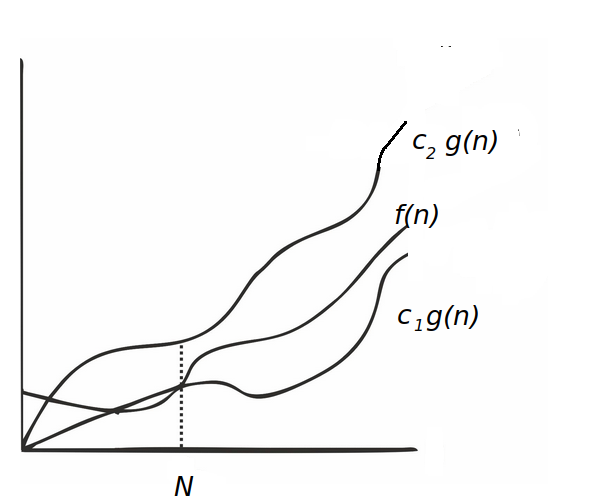
\includegraphics[width=170pt,height=150pt]{slike/theta-notation.png}
	\caption{$\Theta$--notacija: funkcija $f$ je ograničena odozgo i odozdo funkcijom $g$.}
	\label{fig:theta_notation}
\end{figure}

\begin{example}
	Vrijedi 	$T_1(n)=\Theta(n^{3/2}),$ 	dok je $T_2(n)=\Theta(n\log^3 n).$
\end{example}

Pored $O$ i $\Theta$ notacije, često se koriste i $\Omega$ i $o$ notacije.

\begin{definition}
	Neka su date funkcije $f$ i $g$. 	Kažemo da je 	$
	f(n)=\Omega(g(n))$   ako postoje konstante $c>0$ i $N>0$ takve da za svako $n\geq N$ važi $
	f(n)\geq c \cdot g(n).
	$	Funkcija $g$ tada predstavlja asimptotsku donju granicu funkcije $f$.
\end{definition}

\begin{example}
	Vrijedi 	$n^3=\Omega(n^2+n),$ kao i $
	n\log n=\Omega(n).$
\end{example}

\begin{definition}
	Neka su date funkcije $f$ i $g$.
	
	Kažemo da je $
	f(n)=o(g(n))$ ako za svako $c>0$ postoji broj $N>0$ takav da za svako $n\geq N$ važi $0\leq f(n)<c \cdot g(n).$ Drugim riječima, funkcija $f$ raste strogo sporije od funkcije $g$.
\end{definition}

Neformalno posmatrano, uslov $f(n)=o(g(n))
$ znači da odnos $
\frac{f(n)}{g(n)} $ teži nuli kada $n$ teži beskonačnosti.

\begin{example}
	Vrijedi $
	n=o(n^2),
	$ kao i 	$
	n=o(n^3).
	$ 	Međutim, 	$
	n\neq o(n).
	$
\end{example}

Asimptotske notacije predstavljaju osnovni jezik analize algoritama. Njihova najveća prednost ogleda se u tome što omogućavaju poređenje algoritama nezavisno od konkretne implementacije, programskog jezika ili hardverske platforme. Na taj način fokus se prebacuje na fundamentalno pitanje: kako vrijeme izvršavanja raste sa povećanjem veličine ulaza.


\subsection{Neka svojstva $O$--notacije}

Sljedeća teorema navodi nekoliko korisnih pravila koja se često koriste pri računanju asimptotske složenosti algoritama.

\begin{theorem}
	Neka su $f$, $g$ i $h$ pozitivne funkcije definisane za dovoljno velike vrijednosti argumenta. Tada vrijede sljedeće tvrdnje:
	
	\begin{itemize}
		\item $f = O(c \cdot f)$ za svako $c > 0$ \hfill (konstantni faktori su irelevantni);
		
		
		\item Ako je $f = O(g+h)$ i $h = O(g)$, tada je $f = O(g)$ \hfill (pravilo dominantnog člana);
		
		\item $O(f+g)=O(f)+O(g)$ \hfill (pravilo zbira);
		
		\item $O(f\cdot g)=O(f)\cdot O(g)$ \hfill (pravilo proizvoda);
		
		\item Ako je $f=O(g)$ i $g=O(h)$, tada je i $f=O(h)$ \hfill (pravilo tranzitivnosti).
		
		
	\end{itemize}
\end{theorem}

\begin{proof}
	Sve tvrdnje direktno slijede iz definicije $O$--notacije.
\end{proof}

\subsection{Uputstva za procjenu složenosti algoritama}

U prethodnoj sekciji uvedene su osnovne asimptotske notacije koje se koriste za procjenu složenosti algoritama. One omogućavaju da se vrijeme izvršavanja algoritma posmatra kao funkcija veličine ulaza, pri čemu se zanemaruju detalji koji ne utiču značajno na ponašanje algoritma za velike vrijednosti ulaza.

Najčešće funkcije koje se pojavljuju u analizi algoritama prikazane su u Tabeli~\ref{tab:slozenosti_funkcije-a}.

\begin{table}[H]
	\caption{Najčešće klase asimptotske složenosti.}
	\label{tab:slozenosti_funkcije-a}
	\centering
	\begin{tabular}{l|l}
		\hline
		\textbf{Funkcija} & \textbf{Klasa složenosti} \\
		\hline
		$1$ & konstantna  \\ \hline
		$\log n$ & logaritamska \\ \hline
		$n$ & linearna\\  \hline
		$n\log n$ & log-linearna \\ \hline
		$n^2$ & kvadratna \\ \hline
		$n^3$ & kubna \\ \hline
		$2^n$ & eksponencijalna \\ \hline
		$n!$ & faktorijelska \\ \hline
		\hline
	\end{tabular}
\end{table}

Rast navedenih funkcija u zavisnosti od veličine ulaza prikazan je na Slici~\ref{fig:slozenosti_funkcije-a}.

\begin{figure}[H]
	\centering
	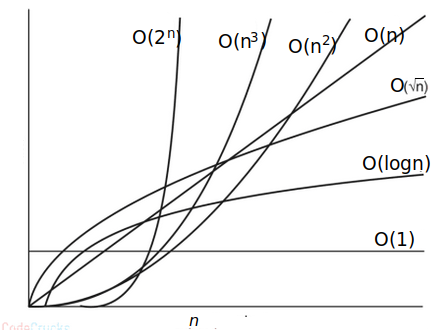
\includegraphics[width=170pt,height=130pt]{slike/growth.png}
	\caption{Poređenje najčešćih klasa složenosti.}
	\label{fig:slozenosti_funkcije-a}
\end{figure}

U praksi se algoritmi eksponencijalne i faktorijelske složenosti smatraju neefikasnim za ulaze velikih dimenzija, jer vrijeme njihovog izvršavanja veoma brzo raste sa povećanjem veličine ulaza. Sa druge strane, logaritamska, linearna i log-linearna složenost najčešće se smatraju poželjnim, budući da omogućavaju obradu veoma velikih instanci problema u razumnom vremenu.

Kvadratna složenost često predstavlja granicu praktične upotrebljivosti algoritma. Za neke probleme ona je sasvim prihvatljiva, dok za druge može biti nedovoljno efikasna, posebno kada se obrađuju veoma veliki skupovi podataka.

U nastavku navodimo nekoliko praktičnih pravila koja olakšavaju procjenu složenosti algoritama. Neka je sa $T(P)$ označena vremenska složenost programa ili programskog segmenta $P$.

\begin{table}[H]
	\caption{Pravila za procjenu složenosti algoritama.}
	\label{tab:uputstva_racunanje}
	\centering
	\begin{tabular}{l|l}
		\hline
		\textbf{Konstrukcija} & \textbf{Složenost} \\
		\hline
		Jedinična instrukcija & $1$ \\
		\hline
		$S: N_1; N_2$ & $T(S)=T(N_1)+T(N_2)$ \\
		\hline
		\textbf{IF} $C$ \textbf{THEN} $N_1$ \textbf{ELSE}  $N_2$ 
		& 
		$T(S)=T(C)+\max\{T(N_1),T(N_2)\}$ \\
		\hline
		\textbf{WHILE} $U$ \textbf{DO} $N_1$
		&
		$T(S)=n\cdot(T(U)+T(N_1))$ \
		\\ \hline
		\textbf{FOR} $i=j$ \textbf{TO} $p$ \textbf{DO} $N_1$
		&
		$T(S)=n\cdot T(N_1)$ \
		\\ \hline
	\end{tabular}
\end{table}

Pri procjeni složenosti algoritama najčešće se zanemaruju konstantni faktori i niži redovi rasta, a pažnja se usmjerava na dominantni član izraza. Na taj način moguće je brzo odrediti asimptotsko ponašanje algoritma bez potrebe za detaljnim brojanjem svih izvršenih instrukcija.\\

Postavlja se pitanje: kada možemo reći da je jedan algoritam efikasniji od drugog?\\


Odgovor daju upravo asimptotske notacije, prvenstveno $O$ i $\Theta$ notacija. Kažemo da je algoritam $X$ \textit{asimptotski efikasniji} od algoritma $Y$ ukoliko za dovoljno velike vrijednosti ulaza vrijeme izvršavanja algoritma $X$ raste sporije od vremena izvršavanja algoritma $Y$.

Drugim riječima, algoritam $X$ pripada nižoj klasi složenosti od algoritma $Y$. Na primjer, algoritam složenosti $O(n\log n)$ asimptotski je efikasniji od algoritma složenosti $O(n^2)$.

Važno je naglasiti da asimptotska efikasnost opisuje ponašanje algoritama za velike vrijednosti ulaza. Za male ulaze moguće je da algoritam sa lošijom asimptotskom složenošću bude brži zbog manjih konstantnih faktora ili jednostavnije implementacije. Ipak, kako veličina ulaza raste, prednost algoritma sa boljom asimptotskom složenošću postaje sve izraženija.


U narednom primjeru razmotrićemo jedan klasičan problem, prikazati dva različita algoritamska pristupa njegovom rješavanju i analizirati njihovu vremensku složenost.

\begin{example}(\textit{Problem podniza maksimalne sume})
	
	Dat je niz brojeva. Potrebno je odrediti neprekidni podniz početnog niza čija je suma elemenata najveća.
\end{example}

\begin{solution}
	
	Neka je dat niz $
	\texttt{a}=[1,4,-2,2,10,-7,1].
	$ 	Primjer jednog neprekidnog podniza jeste $[-2,2,10],$ 	dok niz $[-2,-7,1]$ nije neprekidan podniz jer njegovi elementi nisu uzastopni u izvornom nizu. 	Najprije razmotrimo naivan pristup. Definišimo funkciju
	
	$$
	S(i,j)=\sum_{k=i}^{j} a[k],
	$$
	
	pri čemu je $S(i,i)=a[i]$. 	Dakle, funkcija $S(i,j)$ predstavlja sumu elemenata neprekidnog podniza čiji su početni i završni indeks redom $i$ i $j$.
	
	Za izračunavanje vrijednosti $S(i,j)$ potrebno je sabrati $j-i+1$ elemenata, što zahtijeva $O(n)$ operacija u najgorem slučaju. 	Da bismo pronašli podniz maksimalne sume, potrebno je razmotriti sve moguće parove indeksa $(i,j)$ za koje važi $0 \leq i \leq j < n$. Broj takvih parova jednak je $
	\binom{n}{2}+n=\frac{n(n+1)}{2},
	$ što pripada klasi $O(n^2)$. Kako se za svaki od tih parova funkcija $S(i,j)$ računa u vremenu $O(n)$, ukupna složenost algoritma iznosi $
	O(n)\cdot O(n^2)=O(n^3).
	$	Dakle, dobijamo algoritam koji ima kubnu složenost.
	
	Pokušajmo sada konstruisati efikasniji pristup. Primijetimo da između vrijednosti $S(i,j)$ i $S(i,j+1)$ postoji jednostavna rekurzivna veza	$
	S(i,j+1)=S(i,j)+a[j+1].
	$
	
	Drugim riječima, ukoliko je suma podniza od pozicije $i$ do pozicije $j$ već poznata, suma narednog podniza može se dobiti dodavanjem samo jednog novog elementa. 	Definišimo 	
	$
	S(i)=\max\{S(i,i),S(i,i+1),\ldots,S(i,n-1)\}.$
	
	Vrijednost $S(i)$ može se izračunati prolaskom kroz niz počevši od pozicije $i$, pri čemu se tekuća suma ažurira u konstantnom vremenu. Zbog toga je složenost izračunavanja funkcije $S(i)$ jednaka $O(n)$.
	
	Pošto se funkcija $S(i)$ poziva za svaku početnu poziciju $i \in {0,\ldots,n-1}$, ukupna složenost algoritma iznosi 	$
	n \cdot O(n)=O(n^2).
	$ Time smo složenost smanjili sa $O(n^3)$ na $O(n^2)$, što predstavlja značajno poboljšanje u efikasnosti algoritma.
	
\end{solution}

\section{Prostorna složenost}

Pored vremena izvršavanja, važan kriterijum za procjenu kvaliteta algoritma jeste količina memorije koju algoritam koristi tokom rada.

Pri tome treba razlikovati pojmove \textit{pomoćni prostor} i \textit{prostorna složenost}. Pomoćni prostor predstavlja dodatnu memoriju koju algoritam koristi tokom izvršavanja, ne računajući prostor potreban za smještanje ulaznih podataka.  Sa druge strane, \textit{prostorna složenost} algoritma predstavlja ukupnu količinu memorije potrebne za njegovo izvršavanje, uključujući i prostor za ulazne podatke i pomoćne memorijske strukture.

Kao i kod vremenske složenosti, prostorna složenost izražava se kao funkcija veličine ulaza.  Na primjer:

\begin{itemize}
	\item kreiranje niza dužine $n$ zahtjeva $O(n)$ memorijskog prostora;
	\item kreiranje matrice dimenzija $n \times n$ zahtijeva $O(n^2)$ memorijskog prostora.
\end{itemize}

Efikasnost algoritma najčešće se procjenjuje na osnovu dva kriterijuma: vremena izvršavanja i količine korištene memorije. U mnogim situacijama postoji kompromis između ova dva resursa. Često je moguće ubrzati algoritam korišćenjem dodatne memorije, dok smanjenje memorijskih zahtijeva može dovesti do povećanja vremena izvršavanja.

\begin{example}
	Posmatrajmo sljedeće procedure.
	
	\begin{algorithm}[H]
		\begin{algorithmic}[1]
			\Procedure{pairSum}{x, y}
			\State \textbf{return} $x+y$
			\EndProcedure
		\end{algorithmic}
	\end{algorithm}
	
	\begin{algorithm}[H]
		\begin{algorithmic}[1]
			\Procedure{addSequence}{n}
			\State $sum \gets 0$
			
			\For{$i = 0$ \textbf{to} $n-1$}
			\State $sum \gets sum + \textsc{pairSum}(i,i+1)$
			\EndFor
			
			\State \textbf{return} $sum$
			\EndProcedure
		\end{algorithmic}
	\end{algorithm}
	
	Odredimo prostornu složenost procedure \textsc{AddSequence}.
	
	Iako se funkcija \textsc{pairSum} poziva $O(n)$ puta, ne dolazi do akumuliranja dodatnih memorijskih struktura. Tokom izvršavanja koristi se samo konstantan broj promjenljivih ($sum$, $i$, te parametri funkcije), pa je prostorna složenost algoritma jednaka	$
	O(1).
	$
	
	Drugim riječima, količina memorije ne zavisi od veličine ulaza $n$.
\end{example}

\textbf{Napomena.} 
U praktičnom programiranju raspoloživa memorija je ograničena. Na mnogim sistemima tipična memorijska ograničenja iznose između 128 MB i 512 MB po procesu. Zbog toga nije uvijek moguće kreirati veoma velike nizove ili matrice.

Takođe, lokalne promjenljive funkcija smještaju se na stek, čija je veličina obično znatno manja od ukupne raspoložive memorije procesa. Zbog toga se veoma velike strukture podataka često alociraju u globalnoj memoriji ili na hipu (eng. \emph{heap}), umjesto unutar tijela funkcije.

\section{Pseudok\^od}

\textit{Pseudokod} predstavlja neformalni način zapisivanja algoritama pomoću kombinacije prirodnog jezika i programerskih konstrukcija. Njegova svrha nije da bude izvršiv na računaru, već da na jasan i nedvosmislen način predstavi logiku algoritma.

Za razliku od programskog k\^oda, pseudok\^od ne posjeduje strogo definisanu sintaksu i ne može se kompajlirati niti interpretirati. Upravo zbog toga omogućava da se pažnja usmjeri na suštinu algoritma, bez opterećivanja detaljima konkretnog programskog jezika.

Pseudok\^od predstavlja koristan međukorak između ideje rješenja i njegove implementacije. Njime se opisuje redoslijed koraka koje je potrebno izvršiti kako bi se riješio određeni problem, pri čemu zapis ostaje dovoljno prost da ga mogu razumjeti i osobe koje nisu upoznate sa svim detaljima implementacije.

Prednosti korišćenja pseudok\^oda su višestruke:

\begin{itemize}
	\item Poboljšava čitljivost i razumijevanje algoritma.
	
	\item Omogućava fokusiranje na logiku rješenja umjesto na sintaksu programskog jezika.
	
	\item Predstavlja prirodnu vezu između idejnog rješenja, dijagrama toka i implementacije.
	
	\item Služi kao oblik dokumentacije koji olakšava kasnije održavanje i unapre\-đivanje programa.
	
\end{itemize}

Osnovni cilj pseudokoda jeste da nedvosmisleno opiše svaki korak algoritma. Time se olakšava implementacija i smanjuje vjerovatnoća nastanka grešaka tokom razvoja programa.

Konstrukcija pseudokoda započinje detaljnim razumijevanjem problema koji se rješava. Nakon identifikacije potrebnih koraka, koraci se zapisuju u obliku jednostavnih i jasno formulisanih instrukcija.

Prilikom pisanja pseudokoda preporučuje se pridržavanje sljedećih smjernica:

\begin{itemize}
	\item Koristiti jasne i opisne nazive promjenljivih i funkcija.
	
	\item Svaki korak algoritma opisati dovoljno precizno da ne postoji mogućnost različitog tumačenja.
	
	\item Posebnu pažnju posvetiti uslovima zaustavljanja algoritma.
	
	\item Jasno naglasiti strukturu grananja i petlji korišćenjem uvlačenja naredbi.
	
	\item Izbjegavati nepotrebne implementacione detalje i zadržati fokus na logici rješenja.
	
\end{itemize}

Primjer jednostavnog pseudokoda:

\begin{minted}{text}
	tip = unos sa tastature
	
	ako je tip = "1"
	ispiši "Unesen je broj 1"
	
	ako je tip = "2"
	ispiši "Unesen je broj 2"
\end{minted}

Primijetimo da ovakav zapis ne predstavlja program u konkretnom programskom jeziku, već opisuje logiku koju bi program trebalo da realizuje.

\begin{example}
	Napisati pseudokod za pronalaženje najvećeg elementa niza.
	
	\begin{minted}{text}
		Postavi najveći element na prvi element niza.
		
		Prolazi kroz elemente niza jedan po jedan.
		
		Ako je trenutni element veći od najvećeg do sada 
	        pronađenog,
		    ažuriraj vrijednost najvećeg elementa.
		Kraj prolaska kroz niz.
		
		Prikaži najveći element.
	\end{minted}
	
\end{example}

U nastavku prikazujemo formalniji oblik pseudok\^oda, kakav se često koristi u literaturi iz algoritama. Posmatrajmo algoritam za rješavanje problema podniza maksimalne sume iz prethodne sekcije.

\begin{algorithm}[!ht]
	\caption{Funkcija $S_i(i)$}
	\label{S_i}
	\begin{algorithmic}[1]
		\Procedure{$S_i$}{$i$, $niz$}

		\State $s_{\max} \gets niz[i]$
		\State $s \gets niz[i]$
		
		\For{$j=i+1$ to $n-1$}
		\State $s \gets s + niz[j]$
		
		\If{$s > s_{\max}$}
		\State $s_{\max} \gets s$
		\EndIf
		
		\EndFor
		
		\State \Return $s_{\max}$
		
		\EndProcedure
	\end{algorithmic}
\end{algorithm}

\begin{algorithm}[H]
	\caption{Funkcija $S$}
	\label{S}
	\begin{algorithmic}[1]
		\Procedure{$S$}{$niz$}
		\State $s_{\max} \gets niz[0]$
		
		\For{$i=0$ to $n-1$}
		
		\State $s_i \gets S_i(i,niz)$
		
		\If{$s_i > s_{\max}$}
		\State $s_{\max} \gets s_i$
		\EndIf
		
		\EndFor
		
		\State \Return $s_{\max}$
		
		\EndProcedure
	\end{algorithmic}
\end{algorithm}

Ovakav način zapisivanja pseudokoda predstavlja standard u većini udžbenika i naučnih radova iz oblasti algoritama. Iako je formalniji od prethodnih primjera, i dalje ostaje nezavisan od konkretnog programskog jezika, što omogućava da se algoritam jednostavno implementira u Pajtonu, Javi, C-u, C++-u ili bilo kojem drugom jeziku.

\section{O valjanosti algoritma}

Pored analize vremenske i prostorne složenosti, važno je pokazati da algoritam zaista rješava problem za koji je konstruisan. Drugim riječima, potrebno je dokazati njegovu \textit{valjanost} (ispravnost).

Postoji više pristupa dokazivanju ispravnosti algoritama, među kojima izdvajamo sljedeće:

\begin{itemize}
	\item \textit{Matematički dokaz}. Predstavlja najrigorozniji pristup dokazivanju ispravnosti algoritma. Cilj je pokazati da algoritam za svaki dopustiv ulaz vraća ispravno rješenje problema. Jedna od najčešće korištenih tehnika jeste metoda \textit{invarijante petlje}, koju ćemo razmotriti u nastavku.
	
	\item \textit{Formalna verifikacija}. Podrazumijeva modelovanje algoritma pomoću formalnog jezika i korištenje specijalizovanih alata za automatsku provjeru željenih svojstava. Ovakve metode imaju značajnu primjenu u razvoju kritičnih softverskih sistema, gdje čak i mala greška može imati ozbiljne posljedice.
	
	\item \textit{Testiranje}. Iako ne predstavlja formalni dokaz ispravnosti, testiranje je nezaobilazan korak u razvoju softvera. Pokretanjem algoritma nad velikim brojem pažljivo odabranih testnih primjera može se steći visok stepen povjerenja u njegovu ispravnost.
	
\end{itemize}

%\subsection{Metoda invarijante petlje}

Metoda \textit{invarijante petlje} predstavlja jednu od najvažnijih tehnika za dokazivanje ispravnosti iterativnih algoritama.

\begin{definition}
	Invarijanta petlje je tvrđenje koje važi prije prve iteracije petlje, ostaje tačno nakon svake iteracije i važi u trenutku završetka petlje.
\end{definition}

Dokaz ispravnosti algoritma pomoću invarijante petlje obično se sastoji od tri koraka:

\begin{enumerate}
	\item \textbf{Inicijalizacija}. Pokazuje se da invarijanta važi prije prve iteracije petlje.
	
	\item \textbf{Održavanje}. Dokazuje se da, ukoliko invarijanta važi prije određene iteracije, ona ostaje tačna i nakon izvršavanja te iteracije.
	
	\item \textbf{Završetak}. Nakon izlaska iz petlje koristi se invarijanta kako bi se pokazalo da rezultat koji algoritam vraća zaista predstavlja rješenje problema.
	
\end{enumerate}

Prednost ove metode ogleda se u tome što omogućava formalno dokazivanje ispravnosti algoritama koji koriste petlje, bez potrebe da se zasebno analiziraju svi mogući ulazi.

\begin{example}
	Razmotrimo sljedeći algoritam za određivanje najvećeg zajedničkog djelioca (NZD) dva prirodna broja.
\end{example}

\begin{algorithm}[H]
	\begin{algorithmic}[1]
		\Procedure{NZD}{$n,m$}
		\State $d \gets \min(n,m)$
		\While{$n \bmod d \neq 0$ \textbf{or} $m \bmod d \neq 0$}
		\State $d \gets d-1$
		\EndWhile
		
		\State \Return $d$
		\EndProcedure
	\end{algorithmic}
	\caption{Naivni algoritam za određivanje NZD-a.}
	\label{alg:nzd}
	
\end{algorithm}

Neka je sa $d^*$ označen najveći zajednički djelilac brojeva $n$ i $m$. Posmatrajmo tvrđenje $
d^* \leq d.
$  Pokazaćemo da ono predstavlja invarijantu petlje.

\begin{itemize}
	\item \textbf{Inicijalizacija.} Prije prve iteracije važi $
	d=\min(n,m).
	$
	
	Pošto najveći zajednički djelilac ne može biti veći od manjeg od dva broja, slijedi da je 	$
	d^* \leq d.
	$   Dakle, invarijanta važi prije ulaska u petlju.
	
	\item \textbf{Održavanje.} Pretpostavimo da invarijanta važi na početku neke iteracije. U tijelu petlje vrijednost promjenljive $d$ smanjuje se za jedan.
	
	Sve dok se petlja izvršava, trenutna vrijednost $d$ nije zajednički djelilac oba broja. Budući da je $d^*$ najveći zajednički djelilac, mora važiti 	$
	d^* < d.
	$
	
	Nakon izvršavanja naredbe $d \gets d-1$ i dalje ostaje 	$
	d^* \leq d,
	$ pa je invarijanta očuvana.
	
	\item \textbf{Završetak.} Petlja se zaustavlja kada trenutna vrijednost $d$ dijeli i broj $n$ i broj $m$. Dakle, tada je $d$ zajednički djelilac. 	S druge strane, prema invarijanti petlje važi $
	d^* \leq d.
	$
	
	Pošto algoritam ispituje kandidate silaznim redoslijedom, prvi pronađeni zajednički djelilac mora biti upravo najveći zajednički djelilac. Dakle, 	$
	d=d^*.
	$
\end{itemize}

Time je pokazano da algoritam zaista vraća najveći zajednički djelilac ulaznih brojeva.


U praksi je pronalaženje odgovarajuće invarijante često najzahtjevniji dio dokaza. Kod složenijih algoritama invarijanta može biti veoma komplikovana, pa formalni dokaz postaje težak za izvođenje i razumijevanje. Zbog toga se u razvoju softvera formalni dokazi često kombinuju sa opsežnim testiranjem i empirijskom provjerom ispravnosti.

\section{Euklidov algoritam}

Jedan od najstarijih i najpoznatijih algoritama u matematici jeste \textit{Euklidov algoritam} za određivanje najvećeg zajedničkog djelioca (NZD) dva prirodna broja. Algoritam je dobio ime po starogrčkom matematičaru Euklidu, koji ga je opisao u djelu \textit{Elementi} prije više od dvije hiljade godina.

Osnovna ideja algoritma zasniva se na sljedećem svojstvu:

$$\text{NZD}(a,b)=\text{NZD}(b,a\bmod b).$$

Drugim riječima, najveći zajednički djelilac brojeva $a$ i $b$ jednak je najvećem zajedničkom djeliocu brojeva $b$ i ostatka pri dijeljenju broja $a$ brojem $b$. Ovo svojstvo omogućava da se problem postepeno svodi na manje ulaze, sve dok jedan od tih ulaza ne dobije vrijednost nula.

\begin{algorithm}[H]
	\begin{algorithmic}[1]
		\Procedure{NZD}{$a,b$}
		\While{$b \neq 0$}
		\State $r \gets a \bmod b$
		\State $a \gets b$
		\State $b \gets r$
		\EndWhile
		\State \Return $a$
		\EndProcedure
	\end{algorithmic}
	\caption{Euklidov algoritam.}
	\label{alg:nzd-euclid}
\end{algorithm}

\begin{example}
	
	Odredimo najveći zajednički djelilac brojeva 	$
	a=400$ i $b=24.$ 
\end{example}
	
	\begin{solution}
	Algoritam izvršava sljedeće transformacije: 	$
	(400,24)
	\rightarrow
	(24,16)
	\rightarrow
	(16,8)
	\rightarrow
	(8,0).
	$	Pošto je u posljednjem koraku drugi broj jednak nuli, algoritam se zaustavlja i vraća vrijednost prvog broja. Dakle, $\text{NZD}(400,24)=8.$
\end{solution}


Za razliku od naivnog algoritma iz prethodne sekcije, koji u najgorem slučaju ispituje sve brojeve od $\min(a,b)$ do $1$, Euklidov algoritam veoma brzo smanjuje vrijednosti brojeva nad kojima radi. Zbog toga se u praksi koristi gotovo isključivo Euklidov pristup.

Može se pokazati da broj iteracija Euklidovog algoritma raste proporcionalno logaritmu manjeg od ulaznih brojeva. Preciznije, broj iteracija pripada klasi $O(\log \min(a,b)).$

Pri analizi algoritama često se veličina ulaza ne mjeri samim brojevima $a$ i $b$, već brojem bitova potrebnih za njihov zapis. Ako sa $n$ označimo ukupan broj bitova potrebnih za predstavljanje ulaznih brojeva, tada približno važi $
n \approx \log_2(a)+\log_2(b).
$ Prema tome, broj iteracija algoritma raste linearno u odnosu na veličinu ulaza izraženu u bitovima, odnosno pripada klasi $O(n).
$ Pored male vremenske složenosti, Euklidov algoritam koristi svega nekoliko pomoćnih promjenljivih ($a$, $b$ i $r$), pa je njegova prostorna složenost jednaka $O(1).
$

Zahvaljujući svojoj jednostavnosti i efikasnosti, Euklidov algoritam predstavlja jedan od najvažnijih algoritama u teoriji brojeva i računarstvu. Njegove modifikacije koriste se u brojnim oblastima, uključujući kriptografiju, računarsku algebru i teoriju algoritama.

\textbf{Napomena.}
Valjanost Euklidovog algoritma direktno slijedi iz svojstva $\text{NZD}(a,b)=\text{NZD}(b,a\bmod b),$ koje se primjenjuje u svakoj iteraciji algoritma. Budući da se vrijednost drugog argumenta strogo smanjuje, algoritam se nakon konačnog broja koraka zaustavlja, a posljednja nenulta vrijednost predstavlja najveći zajednički djelilac ulaznih brojeva.

\section{Master teorema}

Kod analize algoritama veoma često se pojavljuju rekurzivne relacije koje opisuju
vrijeme izvršavanja algoritma. Ovakve relacije su naročito karakteristične za
algoritamske paradigme zasnovane na rekurzivnom principu, kao što je paradigma
\emph{podijeli pa zavladaj}.

Pretpostavimo da algoritam problem veličine $n$ dijeli na $a$ podproblema,
pri čemu svaki podproblem ima veličinu približno $n/b$. Pored vremena potrebnog
za rješavanje podproblema, algoritam troši dodatno vrijeme za podjelu problema,
kombinovanje parcijalnih rješenja ili druge operacije. Tada se vremenska
složenost algoritma često može opisati rekurentnom relacijom oblika

\[
T(n)=aT\left(\frac{n}{b}\right)+f(n),
\]

gdje je:

\begin{itemize}
	\item $a \geq 1$ broj podproblema koji se rekurzivno rješavaju;
	\item $b > 1$ faktor za koji se smanjuje veličina svakog podproblema;
	\item $f(n)$ vrijeme potrebno za operacije koje se izvršavaju izvan
	rekurzivnih poziva, kao što su podjela problema ili kombinovanje rješenja.
\end{itemize}

Određivanje asimptotske složenosti ovakvih rekurentnih relacija može biti
zahtjevno. \emph{Master teorema} daje jednostavan način za određivanje
asimptotske složenosti velikog broja rekurzija ovog tipa.

\begin{theorem}[Master teorema]
	Neka je vremenska složenost algoritma opisana relacijom
	
	\[
	T(n)=aT\left(\frac{n}{b}\right)+f(n),
	\]
	
	gdje su $a\geq 1$ i $b>1$ konstante. Vrijednost
	
	\[
	n^{\log_b a}
	\]
	
	predstavlja osnovnu veličinu sa kojom se poredi funkcija $f(n)$.
	
	Tada, u najčešćim slučajevima, vrijedi:
	
	\begin{enumerate}
		\item Ako funkcija $f(n)$ raste asimptotski sporije od
		$n^{\log_b a}$, tada je
		
		\[
		T(n)=\Theta\left(n^{\log_b a}\right).
		\]
		
		\item Ako funkcija $f(n)$ raste istom asimptotskom brzinom kao
		$n^{\log_b a}$, tada je
		
		\[
		T(n)=\Theta\left(n^{\log_b a}\log n\right).
		\]
		
		\item Ako funkcija $f(n)$ raste asimptotski brže od
		$n^{\log_b a}$, tada je, pod odgovarajućim dodatnim uslovima,
		
		\[
		T(n)=\Theta(f(n)).
		\]
	\end{enumerate}
\end{theorem}

Drugim riječima, osnovna ideja Master teoreme jeste poređenje troška
rekurzivnih poziva sa troškom operacija koje se izvršavaju izvan rekurzije.

\begin{example}
	 Neka je data rekurzija
	\[
	T(n)=T\left(\frac{n}{2}\right)+\Theta(1).
	\]
	
	Ovdje je $a=1$, $b=2$ i $f(n)=\Theta(1)$. Pošto je
	
	\[
	n^{\log_2 1}=n^0=1,
	\]
	
	funkcija $f(n)$ ima isti red rasta kao $n^{\log_b a}$. Primjenom drugog
	slučaja Master teoreme dobijamo
	
	\[
	T(n)=\Theta(\log n).
	\]
	
	Dakle, vremenska složenost binarne pretrage je logaritamska.
\end{example}

\begin{example}
%	Kod algoritma sortiranja spajanjem (\emph{merge sort}) niz se dijeli na dva
%	podniza približno jednake veličine. Oba podniza se rekurzivno sortiraju, dok
%	operacija njihovog spajanja zahtijeva linearno vrijeme. 
Neka je data rekurentna relacija
	
	\[
	T(n)=2T\left(\frac{n}{2}\right)+\Theta(n).
	\]
	
	U ovom slučaju je $a=2$, $b=2$ i
	
	\[
	n^{\log_2 2}=n.
	\]
	
	Pošto je $f(n)=\Theta(n)$, primjenjuje se drugi slučaj Master teoreme, pa je
	
	\[
	T(n)=\Theta(n\log n).
	\]
\end{example}

\begin{example}
	%Kod Karacubinog algoritma za množenje cijelih brojeva pojavljuje se rekurzija
	U slučaju rekurzicne relacije
	\[
	T(n)=3T\left(\frac{n}{2}\right)+\Theta(n).
	\]
	
	imamo $a=3$ i $b=2$, pa je
	
	\[
	n^{\log_2 3}\approx n^{1.585}.
	\]
	
	Kako funkcija $n$ raste sporije od $n^{\log_2 3}$, primjenjuje se prvi slučaj
	Master teoreme. Prema tome,
	
	\[
	T(n)=\Theta\left(n^{\log_2 3}\right)
	\approx \Theta\left(n^{1.585}\right).
	\]
\end{example}

Master teorema predstavlja veoma koristan alat za brzu procjenu vremenske
složenosti algoritama zasnovanih na rekurzivnom razlaganju problema. U ovoj
knjizi koristićemo je prvenstveno za analizu jednostavnih algoritama zasnovanih
na paradigmi podijeli pa zavladaj.

Detaljan dokaz Master teoreme, njene preciznije formulacije, dodatni uslovi
primjene i slučajevi koji nisu obuhvaćeni prethodno navedenim pravilima
obrađuju se na naprednijim kursevima iz algoritama i analize algoritama na
višim godinama studija.



\section*{Zadaci}

\begin{enumerate}
	\item Izračunati vremensku složenost sljedećeg programa:
	
	\begin{algorithm}[H]
		\begin{algorithmic}[1]
		\Procedure{Zad1}{$N$}
		    \State $ a \gets  0$
		    \For{$i = 0 \text{ to } N$}
		         \For{$j = N \text{ downto } i$}
		    		\State $a \gets  a + i + j$
		         \EndFor
		     \EndFor
	    \EndProcedure	 	    
		\end{algorithmic}
	\end{algorithm}
\item Izračunati vremensku složenost sljedećeg programa 
	\begin{algorithm}[H]
	\begin{algorithmic}[1]
	 \Procedure{Zad2}{$n$}
		\State $i, j, k \gets  0$
		\For{$i = n / 2 \text{ to } n$}
			\For{$j = 2; j \leq n; j = j * 2$}
				\State $k \gets  k + n / 2$
			\EndFor
		\EndFor
	\EndProcedure	 
	\end{algorithmic}
\end{algorithm}
 \item Izračunati vremensku složenost sljedećeg programa 

	\begin{algorithm}[H]
	\begin{algorithmic}[1]
     \Procedure{Zad3}{$N$}
		\State $a \gets 0, i \gets N$
		\While{$i > 0$}
			\State $a \gets a+ i$
			\State $i \gets i / 2$
		\EndWhile
    \EndProcedure	 
	\end{algorithmic}
\end{algorithm}
 \item Izračunati vremensku složenost sljedećeg programa 

\begin{algorithm}[H]
	\begin{algorithmic}[1]
	 \Procedure{Zad4}{$n$}
		\State $k \gets 3$
		\For{$i=0 \text{ to } n-1$}
		    \State $i \gets i * k$
		\EndFor
	   \EndProcedure
	\end{algorithmic}
\end{algorithm}

 \item Izračunati vremensku složenost sljedećeg programa 

\begin{algorithm}[H]
	\begin{algorithmic}[1]
	\Procedure{Zad5}{$n$}
	  \State $sum \gets 0$
	  \For{$i = 1 \text{ to } n$}
	      \For{$j = 1 \text{ to } i\cdot i$}
	          \If{$j \text{ mod } i == 0$}
	              \For{ $k = 1 \text{ to } j$}
                      \State	$sum \gets sum + 1$
                 
                  \EndFor
              \EndIf
          \EndFor
     \EndFor
    \EndProcedure
	\end{algorithmic}
\end{algorithm}


 
 \item Izračunati (ukupnu) složenost sljedeće rekurzije:

\begin{algorithm}[H]
	\begin{algorithmic}[1]
		\Procedure{bubbleSort}{$arr[],size$}
        \For{$i = 0; i < size-1; ++i$}
 	        \For{$j = 0; j < size-1; ++j$}
 	  
 	 	      \If{$arr[j] > arr[j+1]$}
 		        \State $swap( arr [j] , arr [j+1] )$
 		      \EndIf
 		   \EndFor
 	    \EndFor
		\EndProcedure
	\end{algorithmic}
\end{algorithm}



 
	 
 \item Izračunati složenost sljedeće rekurzije: %https://www.geeksforgeeks.org/analysis-algorithms-set-5-practice-problems/?ref=rp
  
 $$	T(n) = 
 \begin{cases}    
         &3\cdot T(n-1), \text{ako }  n > 0 , \\
         & 1, \text{inače} 
   \end{cases}$$

  \item Izračunati složenost sljedeće rekurzije:

$$	T(n) = 
\begin{cases} 
  		&2T(n-1) - 1, \text{ako } n>0, \\
		& 1, \text{inače}
\end{cases}
$$

\item Izračunati prostornu složenost programa datog sljedećim pseudokodom
%https://www.prepbytes.com/blog/data-structure/space-complexity/

\begin{algorithm}[H]
	\begin{algorithmic}[1]
		\Procedure{sum}{$arr[],N$}
		
		\State  $ans \gets 0$
		\For{$i = 0 \text{ to } N$}
		\State $ans \gets ans+arr[i]$
		\EndFor
		\State ispiši $ans$
		\EndProcedure
	\end{algorithmic}
\end{algorithm}



\item Izračunati prostornu složenost programa datog sljedećim pseudokodom
%https://www.prepbytes.com/blog/data-structure/space-complexity/
 
\begin{algorithm}[H]
	\begin{algorithmic}[1]
	  \Procedure{faktorijel}{$N$}
	  	\State $fact \gets 1$
	  	 \For{$i=1 \text{ to } N $}
	  	   
	  	   \State	$fact \gets fact * i$
	  	 \EndFor
	  	\State \textbf{return} \textit{fact}
	  \EndProcedure
	\end{algorithmic}
\end{algorithm}
 


\end{enumerate}